% Für die Fehlerrechung wird die empirische Standartabweichung
% \begin{equation}
%   \sigma = \sqrt{\frac{1}{n-1} \cdot \sum_{i=1}^n(x_i-\overline{x})^2}
%   \label{eqn:Stdabweichung}
% \end{equation}
% und die Gaußsche Fehlerfortpflanzung
% \begin{equation}
%   u_y = \sqrt{\sum_{i=1}^n\left(\frac{\delta y}{\delta x_i}u_x\right)^2}
%   \label{eqn:gauß}
% \end{equation}
% verwendet.
% \begin{figure}
%   \centering
%   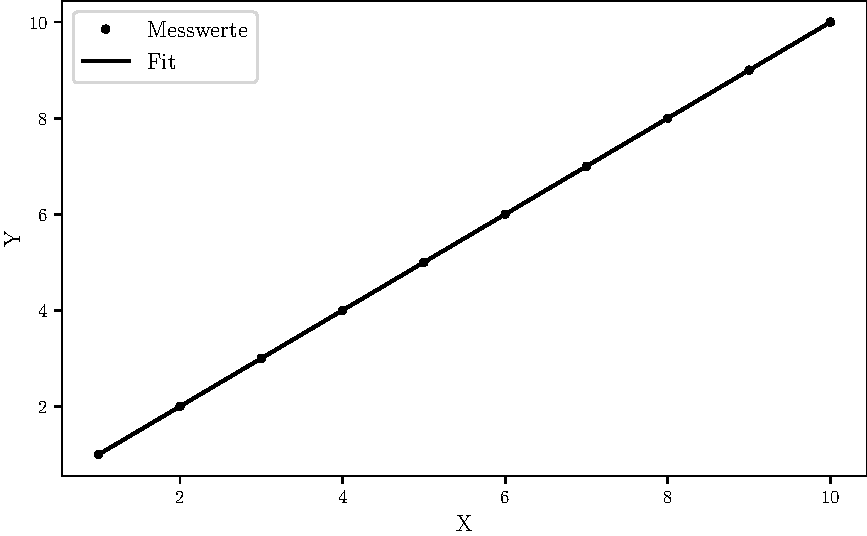
\includegraphics{build/plot.pdf}
%   \caption{Plot}
%   \label{fig:plot}
% \end{figure}
\noindent Die Qualität der Interferenzsignale lässt sich durch den Kontrast $K$
quantifizieren. Um diesen zu ermitteln, wird der initiale Polarisationsfilter
in einem Intervall $\Theta \in [\SI{345}{\degree}, \SI{195}{\degree}]$
in Schritten von je $\theta = \SI{15}{\degree}$ gedreht und die Spannungsextrema
gemessen. Die Messwerte sind in Tabelle \ref{tabular_01} dargelegt. In den
Bereichen um Winkel, an denen der Kontrast besonders auffällig ist, werden
zusätzliche Messungen durchgeführt. 
